% !TeX root = ../thesis.tex

% The second chapter of your thesis.
\chapter{Literature review}

\section{Introduction}

The literature review looks at the impact Asian hornets have on their environment and different methods of tracking Asian hornets with their advantages and disadvantages. Further, we investigate radio telemetry in more detail, look at commercial tag options and end with a conclusion.

\section{Asian hornet}

According to Lioy et al. \cite{lioyInvasiveHornetVespa2022}, the Asian hornet was introduced into northern France by boat in 2004 and subsequently spread throughout northern Europe. The authors note that this invasive species preys on 159 different insects, including honey bees, consuming up to 11.32~kg of insect biomass per season while actively competing with native hornets. Beyond the ecological damage, the invasion carries significant socio-economic consequences. Hornets defending their colonies pose a risk of severe injury or death to humans, and the financial burden of protecting bee populations and managing the invasion can reach 29.5~million euros annually.

The question of how to manage or even if there should be management will not be answered because it is an ongoing debate; however, this thesis will look into how to find hornet nests in a cost-effective and user-friendly way.

\section{Existing Hornet-Tracking Methods}

The ways of tracking hornets can be split into two groups: visual tracking and radio tracking. They each have their own advantages and disadvantages. 

\subsection{Visual Tracking}

Currently, three visual tracking options are commonly used. The first is attaching a lightweight identifier, like reflective tape, to the hornet's waist; this is a cost-effective solution that improves upon tracking with the naked eye, though operators can still easily lose line of sight when the hornet flies out of range \cite{wangReviewFiveExisting2024}. The second option is triangulation, which works by releasing captured hornets from different locations and plotting their flight directions on a map. If the hornets come from the same colony, their flight paths should point to the nest. While this method is intuitive and easy to learn, it is time-consuming, and hornets do not always fly in a straight line to their nest, which can make flight directions inaccurate \cite{wangReviewFiveExisting2024}. The third option is thermal imaging. This works because Asian hornet nests actively regulate their own temperature. A nest becomes visible on thermal images when there is a temperature difference compared to the surrounding environment. This method is most effective in the early morning, without dense tree canopy and when the operator is close to the nest \cite{ViabilityThermalImaging}.

\subsection{Radio Tracking}

The first technique is harmonic radar, which utilizes a lightweight transponder (20~mg) featuring a passive diode that reflects the signal back to the receiver. Operating within the \gls{shf} band, these systems allow for miniature tag dimensions. Harmonic radar determines a target's position by processing the backscattered signal, where time delay indicates range and the angle of arrival provides the direction. Tracking the target across consecutive snapshots reveals both flight trajectory and velocity. The primary limitation of harmonic radar is its high susceptibility to clutter from nearby obstacles, such as dense vegetation or artificial structures, generally restricting reliable operation to open environments \cite{wangReviewFiveExisting2024}.

The final approach is radio telemetry. This method involves mounting a miniature active radio transmitter (less than 200~mg) onto the hornet. The direction is determined using a handheld Yagi antenna, while distance can be found from the \gls{rssi}. The main constraint of radio telemetry lies in the significant design effort required to miniaturize the circuitry and power consumption. Nevertheless, its primary advantage is active signal transmission, which substantially simplifies signal detection and homing \cite{wangReviewFiveExisting2024}.

\subsection{Method Comparison and Selection}

Combining these distinct tracking methodologies can enhance overall search success rates. For instance, active radio telemetry can be deployed for long-range directional tracking, while thermal imaging can be utilized upon reaching the general vicinity to locate the thermal signature of the hidden nest. Consequently, this thesis focuses on the development of an active radio telemetry transmitter to leverage continuous signal broadcasting. This avoids the clutter limitations of harmonic radar in complex terrain, which is essential given that hornet nests are frequently located in woodland and urban environments \cite{lioyInvasiveHornetVespa2022}.

The central engineering challenge lies in balancing competing design requirements: minimizing physical mass and payload volume while maximizing power efficiency and radiated RF output within a single optimized architecture.

\section{Radio-telemetry}

The field of radio telemetry has seen significant evolution since the first radio tag was introduced in 1963 \cite{cochranRadioTrackingSystemWild1963}. This tag (Figure~\ref{fig:wcochran1963sch}) used a single transistor, crystal, capacitor, resistor, loop antenna, and battery to form a transmitter. The loop antenna was used as a collar around the animal being tracked, and the complete tag weighed 10~g.

\begin{figure}[htbp]
	\centering
	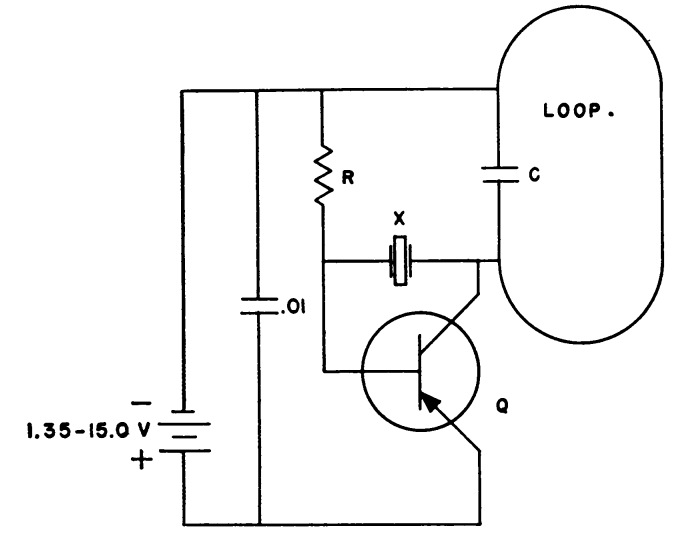
\includegraphics[width=0.7\linewidth]{figs/Wcochran1963sch}
	\caption[Radio-Tracking system for wild animals]{Radio-Tracking system for wild animals \cite{cochranRadioTrackingSystemWild1963}}
	\label{fig:wcochran1963sch}
\end{figure}

This type of transmitter is often called a single-stage tag and operates in the \gls{vhf} band. Cochran's original design transmitted a signal continuously, which is usually unnecessary. Therefore, it is common to modify the circuit with an extra RC network at the base of the transistor to create a pulsing circuit \cite{toledoReviewMiniatureRadio2025}.

While the single-stage tag is simple and requires few components, it has a key flaw: changes in load impedance directly affect the oscillation frequency. This change in impedance occurs when the antenna moves closer to or farther from the animal. Consequently, two-stage tags were developed to improve frequency stability. This extra complexity adds weight to the tag while being a limited improvement for hornet tags.

In recent years, \gls{ble} tags have emerged. They utilize the Bluetooth protocol and can be programmed to distinguish between individual tags. These tags operate at 2.4~GHz, resulting in a much smaller antenna compared to single-stage and two-stage transmitters, but higher frequencies have a limited range and suffer more attenuation from vegetation.

This means that the single-stage tag remains the favorite for small insect trackers due to its low complexity and the ability to use a lower frequency compared to \gls{ble}.

\section{Commercial options}

An important part of the literature study is to find commercial tags and compare them to each other, learn about different technologies that are used in practice, and get an understanding of acceptable prices, ranges, tag weights, and tag dimensions. Different commercial tags are shown in Table~\ref{tab:tracking_tags_comparison}, some purpose-built for tracking hornets while others have more general use cases. The system cost is the price of all the equipment needed to start tracking. The VESPA tracker has the lowest price per tag but lacks in range. The VFT 110 has the lightest tag with a good range and tag price, but the system cost is higher than that of the VESPA and Intuite trackers.

\begin{table*}[htbp]
	\centering
	\caption{Comparison of existing tracking tags suitable for Asian hornets.}
	\label{tab:tracking_tags_comparison}
	\begin{tabular}{l c c c c c}
		\toprule
		\textbf{Tracker} & \textbf{Tag Cost (€)} & \textbf{System Cost (€)} & \textbf{Range (m)} & \textbf{Battery (h)} & \textbf{Weight (mg)} \\
		\midrule
		VESPA tracker & 21.6 & 620 & 500 & 4 & 125 \\
		Intuite & 63 & 348 & 4000 & 4 & 114 \\
		Robor VFT 110 & 49 & 1795 & 2000 & 144 & 110 \\
		Lotek (Nanotag) NTP-1 & 190 & 3215 & 1500 & 288 & 130 \\
		\bottomrule
	\end{tabular}
\end{table*}


\section{Conclusion}

The literature review shows that Asian hornets pose an ecological, economic, and health threat, and an effective method of tracking their nests is essential to protect beehives and human health. While visual tracking and harmonic radar are limited by human eyesight and environmental clutter, the single-stage \gls{vhf} transmitter emerges as the optimal choice. It provides active signal broadcasting while remaining lightweight (<200~mg) with a minimal component count.

Building upon these findings, Chapter 3 details the circuit design, component selection, and SPICE simulations for the \gls{vhf} single-stage transmitter prototype.